\documentclass[11pt]{article}
\usepackage[a4paper,margin=2.5cm]{geometry}
\usepackage[T1]{fontenc}
\usepackage{lmodern}
\usepackage{booktabs}
\usepackage{amsmath}
\usepackage{graphicx}
\usepackage[hidelinks]{hyperref}
\usepackage{natbib}
\graphicspath{{../docs/figures/}}

\title{What Does Analysis of Competing Hypotheses Add to Attack Attribution?\\
\large A Leakage-Controlled Benchmark with Planted, Authentic and Mimicked False Flags}
\author{Rakshit\\Vellore Institute of Technology, Chennai}
\date{Preprint, October 2026 (not peer reviewed)}

\begin{document}
\maketitle

\begin{abstract}
Automated attribution of cyber attacks usually matches observed tactics,
techniques and software against actor profiles. Such matching is easy to
steer: an adversary who plants code, language or metadata artefacts of
another actor can have that actor named. Heuer's Analysis of Competing
Hypotheses (ACH), which ranks hypotheses by how much evidence contradicts
them, is a natural remedy; to our knowledge, automated ACH over ATT\&CK has
not been evaluated against marker-aware baselines and controls. We implement
ACH over MITRE ATT\&CK with mandatory ``unknown actor'' and ``false flag''
hypotheses and evaluate it on 274 held-out ATT\&CK incidents (103 groups) in
five settings: closed world, open world, planted spoofable markers,
\emph{authentic} markers (a false-alarm control) and \emph{mimicry}, where the
adversary copies the framed group's rare techniques as hard evidence. Against
a marker-trusting similarity matcher, ACH reduces the rate at which the framed
group is named from 88.0\% to 1.1\%, but a baseline that ignores spoofable
evidence is never framed, a consistency gate is correct more often under
planted markers (92.0\% vs 73.4\%), and the resistance survives removing all
of ACH's false-flag mechanisms. Under mimicry ACH is framed less often than
IDF coverage (27.0\% vs 32.1\%) but is correct less often (17.9\% vs 28.8\%;
paired difference $-16.0$ to $-6.6$ points). An abstaining similarity baseline
tuned to ACH's closed-world accuracy declines on untracked actors 93.4\% of the
time against ACH's 46.0\%. Under one setting-agnostic calibration map ACH is
less well calibrated overall (pooled Brier 0.214 vs 0.160, paired difference
$+0.031$ to $+0.080$); its advantage is mainly auditability. We release the
benchmark, code and all result files, each tied to the run that produced it.
\end{abstract}

\section{Introduction}
Attribution, deciding who is behind an intrusion, is uncertain and
consequential \citep{rid2015}. Analysts reason from technical evidence whose
reliability varies widely: a rare custom implant is hard to fake, whereas
compiler metadata, language strings and code fragments can be planted
\citep{skopik2020}. Automated attribution systems usually profile actors by
their tactics, techniques and procedures (TTPs) and software and match new
activity to the closest profile \citep{noor2019}. Such matchers inherit the
weakness of the evidence they consume.

Heuer's ACH \citep{heuer1999} asks the analyst to list all reasonable
hypotheses, rate every piece of evidence against every hypothesis, and prefer
the hypothesis with the least inconsistent evidence. False flags are a
recognised problem in the attribution of advanced persistent threats
\citep[Ch.~10]{steffens2020}, and ACH is designed for exactly the case where
some evidence may be deceptive. We ask a narrower, measurable question:
\emph{does automated ACH with mandatory disconfirming-evidence weighting give
better-calibrated, less overconfident attribution than TTP-similarity
matching, especially under false flags, and which of its mechanisms is
responsible?}

\paragraph{Contributions.} (1) An open, leakage-controlled benchmark built
from ATT\&CK \citep{strom2018} with five settings, including an authentic-marker
control and a TTP-mimicry attack, plus campaign, unattributed and temporal
protocols. (2) An auditable ACH engine with span-anchored evidence and
confidence caps. (3) Baselines a reviewer would ask for (spoofable-blind
similarity, IDF coverage, abstention at matched operating points, a
consistency gate) with thresholds cross-fitted by group, one-at-a-time
ablations, a threshold-sensitivity grid, and group-cluster bootstrap
intervals with paired comparisons. (4) A reproduction and ablation of a
published TTP-extraction result \citep{legoy2020}. The novelty claimed is the
measurement, not ACH or false-flag reasoning.

\section{Related work}
\citet{heuer1999} introduced ACH for intelligence analysis. \citet{steffens2020}
covers the attribution of advanced persistent threats, including false flags,
and \citet{rid2015} describe attribution as a layered process that must state
its uncertainty. \citet{skopik2020} survey technical artefacts along the kill
chain and rate how easily each can be spoofed; we use their distinction
between spoofable and hard evidence. The Diamond Model \citep{caltagirone2013}
organises intrusion events by adversary, capability, infrastructure and
victim. \citet{noor2019} profile actors by TTPs and software extracted from
threat reports and attribute them with machine learning; their data and
protocol differ from ours.

Closest to our question, Nunes et al.\ use DEFCON capture-the-flag data, where
the true attacker is known. They find that deceptive activity accounts for
most misattributions by standard classifiers \citep{nunes2015}, and that an
argumentation model in defeasible logic programming, which narrows the set of
candidate culprits, raises classification accuracy from 37\% to 62\%
\citep{nunes2016}. Their data are network traffic from a competition rather
than reported intrusions, their reasoning is argumentation rather than ACH,
and they have no authentic-marker or mimicry controls.

Report-level TTP extraction has been studied by \citet{legoy2020} (rcATT) and
\citet{orbinato2022}. Calibration is measured with the Brier score
\citep{brier1950} and expected calibration error \citep{guo2017}.

\section{Method}
\paragraph{Evidence.} Each evidence row is an observed technique, software,
infrastructure or victim attribute, or a marker (code overlap, language
artefact, metadata, claim) that points at an actor. Markers are typed
spoofable. Rows from text keep the character span they were extracted from,
and every row carries an Admiralty grade.
\paragraph{Hypotheses.} One per candidate actor, one ``false flag: someone
framed $X$'' for each actor a spoofable marker points at, and ``unknown
actor''.
\paragraph{Cells and weights.} Cells take values CC, C, N, I, II. A technique
used by at least 30\% of ATT\&CK groups is non-diagnostic; one used by at most
three groups rates CC on a match; a profile miss is I. Markers support the
matching false-flag hypothesis; hard evidence that contradicts the framed
actor supports the frame. A row's weight is its Admiralty weight times its
diagnosticity (the spread of its ratings across hypotheses); spoofable rows
are multiplied by 0.5.
\paragraph{Ranking and confidence.} Hypotheses are ranked by least weighted
inconsistency; ties go to unknown, then false flag, then a named actor.
Confidence comes from the relative margin and the number of diagnostic rows
and is capped (LOW when support is mostly spoofable; at most MODERATE for
deception or unknown conclusions or when planted-marker indicators fire).

\section{Experimental setup}
\paragraph{Incidents.} Every (group, cited report) pair in ATT\&CK Enterprise
19.2 with at least four techniques or software is an incident (at most three
per group: 274 incidents, 103 groups, 176 candidate profiles). Items cited
only by that report are removed from the group's profile before attribution.
\paragraph{Settings.} \emph{Closed}: the true group is a candidate.
\emph{Open}: it is removed; the correct answer is to decline. \emph{False
flag}: three spoofable markers frame a random other group; naming the true
group or concluding that the framed group was framed counts as correct.
\emph{Authentic}: the same markers point at the true group; concluding a
frame-up is a false alarm. \emph{Mimicry}: the framed group's three rarest
techniques or tools are added as ordinary hard evidence.
\paragraph{Baselines.} IDF-weighted cosine similarity with softmax confidence,
with a marker boost $b$ per marker ($b=0.15$ is the marker-trusting default;
$b=0$ ignores spoofable rows); IDF coverage; similarity that declines below a
cosine threshold $\tau$; and a consistency gate that concludes a frame when
the marker target is not among the top-$k$ groups by hard-evidence similarity.
$\tau$ and $k$ are chosen on one half of the groups and applied to the other
(2-fold, by group). Besides the $\tau$ that maximises mean closed- and
open-world accuracy, two more abstention operating points are cross-fitted to
match ACH: one declines on untracked actors as often as ACH, the other is as
accurate as ACH in the closed world.
\paragraph{Calibration.} A deployed system does not know which setting an
incident comes from, so the main calibration result uses one map (histogram
binning of the stated probability, or a learned grade-to-probability map for
ACH) fitted on closed, open and false-flag incidents together and
cross-fitted by group. Its Brier score is reported for that equal 1:1:1 mix and
per setting; an \emph{overconfident error} is a wrong answer at probability
$\ge 0.8$.
\paragraph{Intervals.} 95\% group-cluster bootstrap intervals (1{,}000
resamples; the incidents of a group are resampled together); paired
differences use the same resamples. A rate of exactly 0 or 1 has a degenerate
bootstrap interval and is given a Wilson interval with the number of groups as
the sample size. Every result file records the code commit and the GitHub
Actions run that produced it; all numbers here come from bench run
37093689060.

\section{Results}
\begin{table}[t]
\centering
\resizebox{\textwidth}{!}{%
\begin{tabular}{lrrrrrr}
\toprule
Method & \multicolumn{2}{c}{Planted markers} & \multicolumn{2}{c}{Authentic markers} & \multicolumn{2}{c}{Mimicry}\\
 & correct & framed & names true & false alarm & correct & framed\\
\midrule
Similarity, $b=0.15$ & 11.3 {\scriptsize[6.4, 16.9]} & 88.0 {\scriptsize[82.3, 93.3]} & 100.0 {\scriptsize[96.4, 100.0]}$^\dagger$ & 0.0 {\scriptsize[0.0, 3.6]}$^\dagger$ & 21.2 {\scriptsize[15.5, 27.0]} & 76.3 {\scriptsize[70.9, 81.8]} \\
Similarity, $b=0.05$ & 49.6 {\scriptsize[41.9, 57.3]} & 12.4 {\scriptsize[8.5, 16.9]} & 85.4 {\scriptsize[80.4, 90.4]} & 0.0 {\scriptsize[0.0, 3.6]}$^\dagger$ & 21.2 {\scriptsize[15.5, 27.0]} & 76.3 {\scriptsize[70.9, 81.8]} \\
Similarity, $b=0$ & 53.3 {\scriptsize[45.3, 60.8]} & 0.0 {\scriptsize[0.0, 3.6]}$^\dagger$ & 53.3 {\scriptsize[45.3, 60.8]} & 0.0 {\scriptsize[0.0, 3.6]}$^\dagger$ & 21.2 {\scriptsize[15.5, 27.0]} & 76.3 {\scriptsize[70.9, 81.8]} \\
IDF coverage & 42.0 {\scriptsize[34.5, 49.1]} & 0.0 {\scriptsize[0.0, 3.6]}$^\dagger$ & 42.0 {\scriptsize[34.5, 49.1]} & 0.0 {\scriptsize[0.0, 3.6]}$^\dagger$ & \textbf{28.8} {\scriptsize[21.9, 35.8]} & 32.1 {\scriptsize[25.4, 39.2]} \\
Similarity + abstain & 26.6 {\scriptsize[19.6, 33.8]} & 0.0 {\scriptsize[0.0, 3.6]}$^\dagger$ & 26.6 {\scriptsize[19.6, 33.8]} & 0.0 {\scriptsize[0.0, 3.6]}$^\dagger$ & 10.9 {\scriptsize[6.7, 15.4]} & 44.5 {\scriptsize[38.5, 50.4]} \\
Consistency gate & \textbf{92.0} {\scriptsize[88.4, 95.2]} & 8.0 {\scriptsize[4.8, 11.6]} & 77.0 {\scriptsize[70.8, 83.3]} & 23.0 {\scriptsize[16.7, 29.2]} & 21.2 {\scriptsize[15.5, 27.0]} & 76.3 {\scriptsize[70.9, 81.8]} \\
OCCAM ACH & 73.4 {\scriptsize[66.9, 79.6]} & 1.1 {\scriptsize[0.0, 2.6]} & 35.8 {\scriptsize[28.8, 42.6]} & 18.6 {\scriptsize[13.8, 24.4]} & 17.9 {\scriptsize[12.2, 23.8]} & \textbf{27.0} {\scriptsize[21.3, 33.5]} \\
\bottomrule
\end{tabular}}
\caption{False-flag settings, 274 incidents, 3 markers or mimicked items;
percent with 95\% group-cluster bootstrap intervals ($^\dagger$: Wilson
interval with the 103 groups as the sample size, for a rate of exactly 0 or
100\%). Source: \texttt{results/falseflag.json}.}
\label{tab:ff}
\end{table}

\begin{table}[t]
\centering
\resizebox{\textwidth}{!}{%
\begin{tabular}{lrrrr}
\toprule
Method & Closed: correct (\%) & Open: correct decline (\%) & Brier, pooled map & ACH minus method\\
\midrule
Similarity, $b=0.15$ & 53.3 {\scriptsize[45.3, 60.8]} & 0.0 {\scriptsize[0.0, 3.6]}$^\dagger$ & 0.160 {\scriptsize[0.141, 0.178]} & [+0.031, +0.080] \\
Similarity, $b=0$ & 53.3 {\scriptsize[45.3, 60.8]} & 0.0 {\scriptsize[0.0, 3.6]}$^\dagger$ & 0.151 {\scriptsize[0.128, 0.173]} & [+0.039, +0.087] \\
IDF coverage & 42.0 {\scriptsize[34.5, 49.1]} & 0.0 {\scriptsize[0.0, 3.6]}$^\dagger$ & 0.167 {\scriptsize[0.143, 0.192]} & [+0.021, +0.074] \\
Consistency gate & 53.3 {\scriptsize[45.3, 60.8]} & 0.0 {\scriptsize[0.0, 3.6]}$^\dagger$ & 0.204 {\scriptsize[0.190, 0.217]} & [$-$0.005, +0.027] \\
Abstain, $\tau$ for closed + open & 26.6 {\scriptsize[19.6, 33.8]} & 94.5 {\scriptsize[92.0, 97.1]} & 0.214 {\scriptsize[0.203, 0.226]} & [$-$0.016, +0.017] \\
Abstain, $\tau$ matched to ACH's declines & 47.4 {\scriptsize[39.7, 55.0]} & 47.8 {\scriptsize[41.8, 53.5]} & 0.208 {\scriptsize[0.191, 0.224]} & [$-$0.014, +0.027] \\
Abstain, $\tau$ matched to ACH's accuracy & 29.9 {\scriptsize[22.7, 37.4]} & 93.4 {\scriptsize[90.6, 96.1]} & 0.214 {\scriptsize[0.202, 0.227]} & [$-$0.016, +0.017] \\
OCCAM ACH & 29.9 {\scriptsize[22.9, 37.1]} & 46.0 {\scriptsize[39.3, 53.1]} & 0.214 {\scriptsize[0.202, 0.226]} & --- \\
\bottomrule
\end{tabular}}
\caption{Closed and open world, and calibration under one setting-agnostic
map fitted on closed + open + false-flag incidents (822 answers; lower Brier is
better). Last column: paired 95\% interval of ACH's Brier minus the method's.
Source: \texttt{results/falseflag.json}.}
\label{tab:open}
\end{table}

\paragraph{Planted markers.} Table~\ref{tab:ff}: the marker-trusting matcher
names the framed group 88.0\% of the time, ACH 1.1\% (95\% CI 0.0--2.6\%). The
result depends on how strongly the matcher trusts markers: at $b=0.05$ it is
framed 12.4\% of the time and at $b=0$ never. The consistency gate is correct
92.0\% of the time against ACH's 73.4\% (paired difference $-25.6$ to $-12.2$
points).
\paragraph{Authentic markers.} With genuine markers ACH calls the overlap a
frame-up in 18.6\% of incidents (CI 13.8--24.4\%) and names the true group only
35.8\% of the time; the marker-trusting matcher names it 100\%.
\paragraph{Mimicry.} When the adversary copies the framed group's rarest
techniques as hard evidence, nothing is pre-typed as spoofable and the gate
cannot help. TTP similarity names the framed group 76.3\% of the time, IDF
coverage 32.1\% and ACH 27.0\% (paired difference to coverage $-8.6$ to
$-1.8$ points). ACH is, however, \emph{correct} less often than coverage:
17.9\% against 28.8\% (paired $-16.0$ to $-6.6$ points); against plain
similarity (21.2\%) the difference is not significant ($-10.1$ to $+3.5$).
With six mimicked items ACH is framed 44.2\% of the time against 90.9\% for
similarity. The gain is not specific to ACH's weighting: without diagnosticity
weighting ACH is framed less under mimicry (18.2\%), at a cost in closed-world
accuracy, and support-aware ranking is framed more (35.4\%).
\paragraph{Ablations.} Removing the false-flag hypotheses leaves ACH's framed
rate at 1.1\% and raises ``names the true group'' from 2.2\% to 20.1\%;
removing the hypotheses, the 0.5 spoofable discount and the caps together
leaves it at 2.6\%; removing only the discount changes accuracy by under two
points. Resistance to planted markers therefore survives removing every
false-flag-specific mechanism: it comes from hard evidence contradicting the
framed group, which both ranking rules honour (support-aware ranking is framed
1.5\% of the time). For the baselines, ignoring spoofable rows is sufficient.
The false-flag hypotheses convert outcomes into explicit ``framed''
conclusions. The confidence caps change no accuracy metric and do not improve
calibration: pooled Brier is 0.214 with them and 0.207 without (variant minus
full ACH $-0.010$ to $-0.005$), whereas removing the spoofable discount
worsens it to 0.231. Removing the unknown hypothesis raises closed-world
accuracy from 29.9\% to 37.2\% but removes all declines.

\begin{figure}[t]
\centering
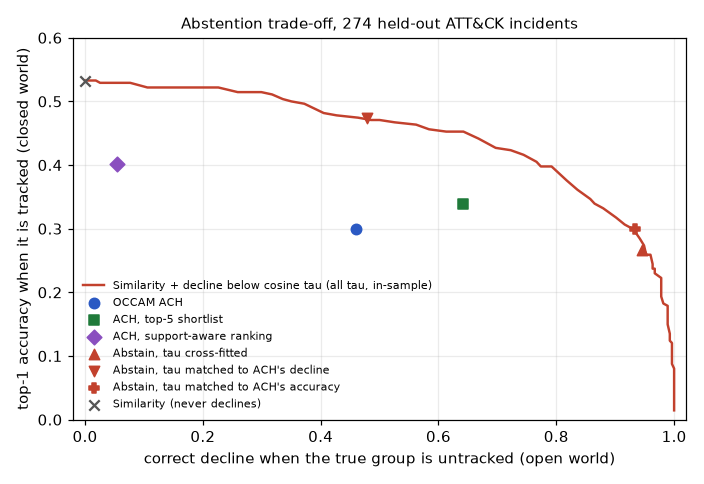
\includegraphics[width=0.78\textwidth]{abstention_frontier.png}
\caption{Abstention trade-off on the 274 incidents. Red curve: the cosine
threshold baseline over all $\tau$ (in-sample); markers: cross-fitted
operating points and ACH variants. Every ACH variant lies inside the
baseline's frontier. Source: \texttt{results/falseflag.json}.}
\label{fig:frontier}
\end{figure}

\paragraph{Closed and open world.} Table~\ref{tab:open} and
Figure~\ref{fig:frontier}. Similarity names the true group 53.3\% of the time
and ACH 29.9\%. When the true group is untracked ACH declines 46.0\% of the
time, and 36.5\% of the time when it is tracked. The abstaining baseline does
better at either matched operating point: as accurate as ACH in the closed
world, it declines 93.4\% of the time (paired $-54.8$ to $-39.6$ points);
declining as often as ACH, it is right 47.4\% of the time in the closed world
(paired $-25.4$ to $-10.0$). Because it ignores rarity, the same baseline is
framed more under mimicry (44.5--71.5\% across its operating points).
\paragraph{Calibration and overconfidence.} With one setting-agnostic map,
ACH's Brier score over the three settings is 0.214 against 0.160 for the
marker-trusting matcher (paired difference $+0.031$ to $+0.080$). Per setting,
ACH is better in the closed world (0.189 vs 0.315; $-0.178$ to $-0.075$) and
worse in the open (0.249 vs 0.032) and false-flag settings (0.205 vs 0.131),
so the pooled number depends on the 1:1:1 mix. One map cannot help similarity,
which never declines: its open-world answers are all wrong, the map lowers
every probability, and its closed-world Brier rises from 0.179 uncalibrated to
0.315. Overconfidence is a property of the raw outputs: under planted markers
ACH's capped grades are never wrong at stated $p \ge 0.8$ (0 of 274), while the
matcher's softmax is (194 of 274). After the setting-agnostic recalibration
neither makes such errors (ACH 1 of 822, similarity 0 of 822). Brier alone does
not measure framing resistance: a matcher with marker boost 0.3 is framed in
every planted-marker incident yet has the lowest pooled Brier (0.124), because
it states low probabilities.
\paragraph{Threshold sensitivity.} The cell-rule thresholds (30\% of groups,
three groups) were set by hand. Over a $3\times3$ grid (20/30/40\%; 2/3/5
groups), closed-world accuracy ranges 27.0--35.4\%, correct declines
36.9--59.1\%, framing under planted markers 0.7--1.1\%, false alarms
15.0--27.4\% and framing under mimicry 24.8--36.1\%. Choosing the thresholds
on one group fold and applying them to the other selects the 20\% cut-off,
which raises closed-world accuracy by 4.0 points (paired $+1.5$ to $+6.9$) but
also false alarms ($+4.2$ to $+10.8$) and mimicry framing ($+5.3$ to $+12.4$).
\paragraph{Larger and later data.} Over all 575 report incidents, 21 held-out
campaigns and temporal splits (profiles from ATT\&CK v12.1 or v15.1,
activity added afterwards, renamed technique ids mapped back), the open-world
and planted-marker comparisons with the naive matcher point the same way; in
the closed world ACH is lower on the 575 incidents (39.0\% vs 47.8\%) and both
methods are weak in the temporal splits (v12.1: 21.3\% vs 20.2\%). ACH declines
50.6\% of the time in the v12.1 split when the group is removed. The authentic,
mimicry and simple-baseline controls were run only on the 274-incident set.
\paragraph{Real reports.} On 75 APTnotes reports labelled by file name and
title, with ATT\&CK citations that match the report held out, ACH's top-1
accuracy is 32.0\% (Wilson CI 23--43\%) against 28.0\% for similarity; 12
reports are correct only for ACH and 9 only for similarity (exact McNemar
$p=0.66$). No ACH answer is wrong at stated probability $\ge 0.8$ (similarity:
9 of 75), but this holds almost by construction, because ACH's grades are
capped (HIGH, 0.875, is rarely reachable; answers are capped at MODERATE,
0.675, whenever deception indicators fire or a same-actor false-flag
hypothesis is not rejected). Adding the TF-IDF sentence classifier (top 10
techniques per report) lowers ACH to 16.0\%: 12 reports lost, none gained
($p=0.0005$); similarity is unchanged (29.3\%, $p=1.0$). Attributing on
software names alone gives 48.0\% for similarity and 45.3\% for ACH; techniques
alone are near zero.
\paragraph{Reproduction.} The rcATT paper reports tactic micro-F$_{0.5}$
$65.38\pm2.87$ and technique micro-F$_{0.5}$ $35.02\pm5.32$
\citep[Table~4, ``Inde.'' rows; the same means are in Tables~2 and 3]{legoy2020}.
On rcATT's 1,490 reports with the released code's 5-fold split, the released
code gives $64.82\pm3.44$ and, for the 197 techniques that the paper's
at-least-5-reports filter keeps in the released data, $36.33\pm1.39$. The
released code differs from the paper text in two undocumented settings,
stemming/lemmatisation and balanced class weights. A $2\times2$ ablation on
the same folds attributes most of the technique difference to class
weighting ($+5.9\pm2.5$ points, fold-paired) and little to tokenisation
($+0.3\pm0.6$); the paper-text pipeline reaches 29.28. For tactics, balanced
weights slightly lower micro-F$_{0.5}$ ($-1.7\pm0.9$). OCCAM's TF-IDF +
logistic regression gets 34.18 micro but 12.94 macro F$_{0.5}$ on the same
folds: it is not better than rcATT on this task.

\section{Discussion and conclusion}
The research question asked whether automated ACH gives better-calibrated,
less overconfident attribution than TTP-similarity matching under false
flags. On this benchmark the answer is mostly no.
\emph{Calibration}: under one setting-agnostic map ACH is less well calibrated
overall (pooled Brier 0.214 vs 0.160, $+0.031$ to $+0.080$); it is better
only in the closed world.
\emph{Overconfidence}: ACH's capped grades are never confidently wrong under
planted markers, where the matcher's softmax often is, but after one
recalibration neither method makes such errors, so the difference lies in the
raw outputs rather than in the ranking.
\emph{Framing}: the rate at which planted markers get the framed group named
falls from 88.0\% to 1.1\%, but baselines that ignore spoofable evidence match
it, and ACH's own false-flag machinery is not what produces it.
\emph{Mimicry}: ACH is framed somewhat less often than IDF coverage but is
correct less often.
\emph{Abstention}: a thresholded similarity baseline declines more at similar
closed-world accuracy, and ACH's operating point lies inside its frontier.
What remains is auditability: every ACH conclusion comes with a matrix of
span-anchored evidence that an analyst can inspect and override. That is a
design property, not a measured one; measuring whether it helps analysts
would need a user study. For practitioners, the actionable findings are
simpler: type evidence by spoofability, let a model decline, and do not read a
low Brier score as resistance to framing.

\section{Limitations}
False-flag evidence is synthetic: markers and mimicked items are evidence
rows, not forged binaries. Incidents are slices of ATT\&CK's reading of
public reporting rather than telemetry. The APTnotes set is small and its
leak control is a title-matching heuristic. ACH rarely names the true actor
behind a detected frame (2.2\%), and its closed-world accuracy is well below
plain similarity. The cell-rule thresholds were set by hand; the sensitivity
grid shows the trade-offs they encode. The pooled calibration result assumes
an equal mix of the three settings. Auditability, the advantage we claim for
ACH, is not measured.

\section{Ethics and reproducibility}
Attribution affects people and states; OCCAM is decision support and every
output says so. Results about real ATT\&CK groups are benchmark artefacts, not
findings. No malware was downloaded or executed; all data are public, pinned
to commits and checksummed. Every result file records the commit, command,
package versions, input checksums and GitHub Actions run that produced it, and
a manual workflow regenerates all results and lists any value that changed.
Code, result files and exact commands are at
\url{https://github.com/rakshit-737/occam-cti-attribution}.

\section*{Acknowledgements}
The code, experiments and this text were developed with AI assistance
(Claude, Anthropic). Every DOI, arXiv identifier and URL in the bibliography
was resolved and compared with its entry by a script whose log is in the
repository (\texttt{paper/refs\_check.log}). The author is responsible for all
claims.

\bibliographystyle{plainnat}
\bibliography{refs}
\end{document}
